\chapter{A Dynamic Navigation Model for Co-located Collaboration}
\label{chapter:dynamic_model}
\pagebreak

\textbf{Chapter Abstract}

This chapter presents a novel dynamic navigation model named DYNAMIC that we designed for co-located collaboration. This model allows more advanced navigation control by integrating constrains from physical workspace and the virtual world. We first explained our motivation and different components of DYNAMIC at a conceptual level, then we presented implementation details from data structure to code organization, as well as some discussion about possible improvements.

\vspace*{2\baselineskip}

\minitoc

\newpage
\section{Introduction}
The Altered Human Joystick metaphor allows individual navigation for multiple users, however, each user is constrained in a predefined safe zone and the common workspace is shared by using a system dependent protocol (which works for cubic immersive systems). Moreover, in many rate control navigation metaphors, the virtual vehicle's velocity is exclusively controlled by user's input and can not be influenced by constrains from the virtual world (e.g. collisions with objects). 

To generalize the Altered Human Joystick metaphor and to allow interactive control of the virtual vehicle, we designed a dynamic navigation model named DYNAMIC (DYnamic NAvigation Model for Immersive Collaboration), which on the one hand, integrates real world information into the virtual navigation control to manage user cohabitation no matter the geometric properties of the immersive system, and on the other hand, takes into account influences coming from the virtual world and eventually from the vehicles of other users.

This chapter mainly contains four sections. The first section explains our motivation of developing this dynamic navigation model. The second part describes core concepts of this model: the acceleration-based transfer function and how we integrate constrains coming from the physical workspace and the virtual world. Then the third section presents implementation details and the last one some related discussion about this navigation model.


% -------------------------------------------------------------------------------------------------

\section{Motivation}
The dynamic navigation model is the result of responses to two different research questions that we are working on: how can we generalize the Altered Human Joystick metaphor to extend the number of users regardless of the geometric configuration of immersive systems? And how can we make the virtual vehicle to be responsive to constrains coming from the virtual world to achieve interactions with virtual objects and other users during navigation?

In this dynamic model, the transfer functions used in human joystick metaphors are replaced by their derivatives so the vehicle is controlled by accelerations instead of specifying directly its navigation velocity. As a consequence, the virtual vehicle is transformed from a pure reference frame to a virtual entity possessing its own kinematic state, providing a uniform interface to receive inputs from various sources. First, to integrate constrains from the physical workspace, we use a potential field method which generates accelerations for the virtual vehicle in order to influence user's navigation control. Second, virtual vehicles can now react to constrains in the virtual worlds in form of physical links. We can simulate physical interactions between a vehicle and virtual objects, or directly between different users' vehicles during navigation. 


% -------------------------------------------------------------------------------------------------


\section{Concepts}

\subsection{Transfer Function}
The original human joystick metaphor and the altered versions that we present in the previous chapter are based on transfer functions that map a user's relative position and orientation related to a neutral reference frame to the vehicle's translation and rotation velocities. In this case, a neutral position and orientation $(p_{0},q_{0})$ need to be defined before starting navigation. The vehicle's translation and rotation velocity are expressed as:

\begin{equation}
\label{eq:old_tf_t}
\overrightarrow{v_{veh}}=f(\Delta p)=f(p_{u}-p_{0})
\end{equation}
\begin{equation}
\label{eq:old_tf_r}
\Omega_{veh}=f(\Delta q)=f(q_{u}-q_{0})
\end{equation}

where $p_{u}$ is user's current position and $q_{u}$ is a quaternion representing user's orientation in the real world.

In the dynamic model, the virtual vehicle is not merely a spatial reference frame, but a virtual entity possessing its own kinematic state. The user input passes from $(\Delta p, \Delta q)$ to their derivatives: 

\begin{equation}
\overrightarrow{a_{veh}}=f(\overrightarrow{v_{u}}, \overrightarrow{a_{u}})
\end{equation}
\begin{equation}
\dot{\Omega}_{veh}=f(\omega_{u}, \dot{\omega}_{u})
\end{equation}

If we define a configuration \textit{c} as the following:

\begin{equation}
c=
\begin{bmatrix}
p \\ q
\end{bmatrix},\:
\dot{c}=
\begin{bmatrix}
\overrightarrow{v} \\ \omega
\end{bmatrix},\:
\ddot{c}=
\begin{bmatrix}
\overrightarrow{a} \\ \dot{\omega}
\end{bmatrix}
\end{equation}

to have a uniform representation of linear and angular information, where $\dot{c}$ and $\ddot{c}$ are the first and second temporal derivatives of \textit{c}. A linear version of the new transfer function can be then expressed as:

\begin{equation}
\ddot{c}_{veh}=K_{1} \cdot \dot{c}_{u} + K_{2} \cdot \ddot{c}_{u}
\end{equation}

\begin{equation}
\begin{bmatrix}
\overrightarrow{a_{veh}} \\ \dot{\omega}_{veh}
\end{bmatrix}=
\begin{bmatrix}
K_{T1} & 0 \\ 0 & K_{R1}
\end{bmatrix}
\begin{bmatrix}
\overrightarrow{v_{u}} \\ \omega_{u}
\end{bmatrix} + 
\begin{bmatrix}
K_{T2} & 0 \\ 0 & K_{R2}
\end{bmatrix}
\begin{bmatrix}
a_{u} \\ \dot{\omega}_{u}
\end{bmatrix}
\end{equation}

Instead of setting directly the vehicle's position or velocity in the virtual world, user's physical movements ``inject" accelerations to animate the virtual vehicle. This transfer function allows easy integration of physical constrains into the vehicle control. Moreover, the navigation velocity no longer depends on user's real world configuration, neither do we need a predefined neutral reference frame.


\subsection{Physical Workspace Constrains}
In a multi-user immersive system, for a given user, the surrounding environment as well as other users are obstacles that should be avoided. In the domain of robotics, potential field is used to guide a robot to navigate over a field occupied by obstacles to get to a target position. Generally, two kinds of potential fields lead to two different behaviors of the robot. An attractive field generates an action vector that leads the robot toward the goal, while a repulsive field pushes the robot away from an obstacle.

Here we want to use the same principle to guide users by applying repulsive fields to all obstacles in the real world (e.g. screens, walls, other users, etc.). The goal is to keep users away from all the obstacles when they move around in the physical workspace. However, the big ``problem" is that unlike motor-driven robots, users are autonomous actors that can not be directly influenced by the potential field. So, like the divergent transfer function described in the previous chapter (section~\ref{sec:altered_tf}), we modify the output of the transfer function (i.e. $\overrightarrow{a_{veh}}$) by integrating obstacles as real world constrains into the navigation control in order to influence user's input (i.e. $\overrightarrow{v_{u}}$ and $\overrightarrow{a_{u}}$).


\subsubsection{Potential Field}
To achieve the above objective, obstacles generate one potential field for a user's translational movements and another for rotations. The workspace borders are usually fixed while the users are mobile entities, so the global potential fields change dynamically according to users' positions in the physical workspace.

\paragraph{Translational Field}
To avoid collisions between users and to prevent them from going beyond workspace borders, each physical obstacle produces a repulsive field in which force vectors are in the direction of the surface normal, thus the distribution of potential field depends on obstacles' geometric form. For example, the potential field of a flat wall or screen generates parallel force vectors while those of a user's field (the user is simplified as a cylinder) spread outward from user's position (Figure~\ref{fig:5_pf_t}).

\begin{figure}[htb]
  \centering
  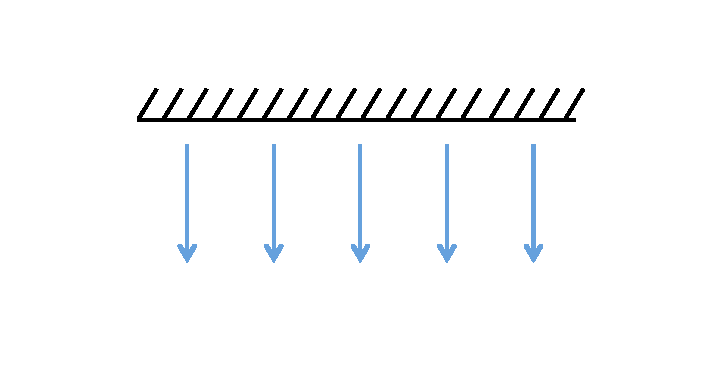
\includegraphics[width=.49\textwidth]{figures/ch5/pf_t_wall}
  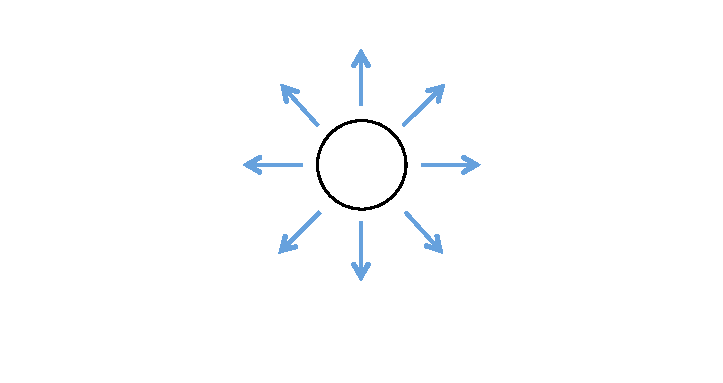
\includegraphics[width=.49\textwidth]{figures/ch5/pf_t_user}
  \caption{\label{fig:5_pf_t}The repulsive translational potential fields generated by obstacles.}
\end{figure}

If we name $\overrightarrow{n}_{i}$ as a unit surface normal vector, $d_{i}$ the distance between a user and the obstacle $i$, the force vector generated for the user $\overrightarrow{ft}_{i}$ can be expressed by a negative exponent function:

\begin{equation}
\overrightarrow{ft}_{i}=\overrightarrow{n}_{i} \cdot K_{T} \cdot \frac{1}{d_{i}^2}
\end{equation}

where $K_{T}$ is a coefficient to modulate the field power.

\paragraph{Rotational Field}
In projection-based systems, the rotational potential field can help users avoid seeing empty screens and occlusions. Even with HMDs, rotational fields are still useful if we want to influence a user's orientation in the physical workspace. Rotational potential field works in a similar way as for translation, obstacles provide forces to make a user to turn towards one direction or another (clockwise or anti-clockwise). The potential fields associated with screen edges help user stay within projected area, while the potential field of a user pushes other users to look away (Figure~\ref{fig:5_pf_r}).

\begin{figure}[htb]
  \centering
  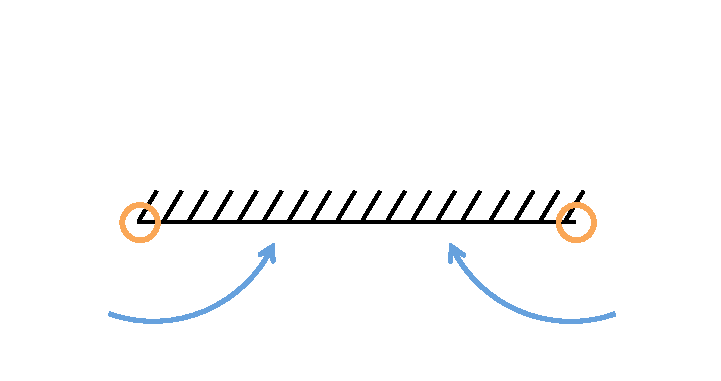
\includegraphics[width=.49\textwidth]{figures/ch5/pf_r_wall}
  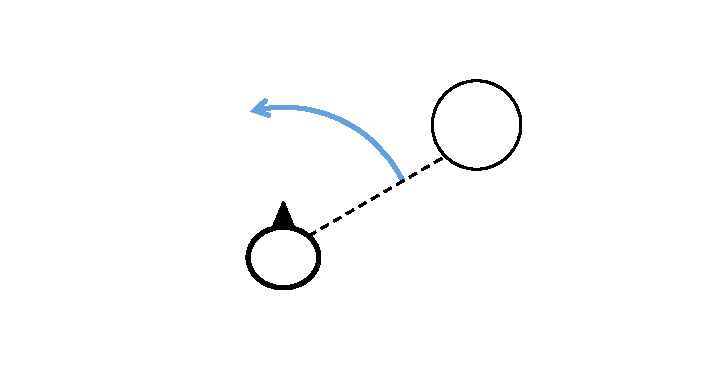
\includegraphics[width=.49\textwidth]{figures/ch5/pf_r_user}
  \caption{\label{fig:5_pf_r}The repulsive rotational potential field generated by obstacles.}
\end{figure}

We can name $sign \in \{-1, 1\}$ to indicate the rotation direction (computed using user's orientation compared to the direction vector $\overrightarrow{P_{u}P_{o}}$, $P_{u}$ and $P_{o}$ are respectively the user's and obstacle's position). $\theta_{i}$ is the angle that the user needs to cover starting from the current orientation till seeing the obstacle $i$, then the force vector generated for the user $\overrightarrow{fr}_{i}$ can be expressed by a negative exponent function:

\begin{equation}
{fr}_{i}=sign \cdot K_{R} \cdot \frac{1}{\theta_{i}^2}
\end{equation}

where $K_{R}$ is a coefficient to modulate the field power.

\subsubsection{Solutions}
With the above potential fields associated with each obstacle, users will naturally keep a distance with all obstacles no matter the system configuration, which means we no longer need to specify particular working zones or shared zone for each user as we did in Chapter~\ref{chapter:user_cohab}. So now the question is how users can ``perceive" and be influenced by the potential fields.

\paragraph{Optimal Configuration} In a physical workspace filled with several obstacles, the global potential field for a user is the combination of potential fields of all obstacles, and each user will have a different potential field distribution since he/she is considered as an obstacle for the other users. For each user, the superimposed potential fields result in one or several (local minimum values) special positions and orientations where the forces are neutralized. We can use optimal configuration $c_{opt}$ to denote the combination of optimal position and orientation:

\begin{equation}
c_{opt}=
\begin{bmatrix}
p_{opt} \\ q_{opt}
\end{bmatrix}
\end{equation}

where

\begin{equation}
\sum \overrightarrow{ft}_{i}=(0, 0)\; and\; \sum fr_{i}=0
\end{equation}


Figure~\ref{fig:5_pf_total} shows an example inside a three-wall CAVE, the final potential field for user A is the combination of the fields of other two users and those of all physical borders (a virtual back wall is added to assure users in the range of the screen floor). Optimal position and orientation are marked by green color.

\begin{figure}[htb]
  \centering
  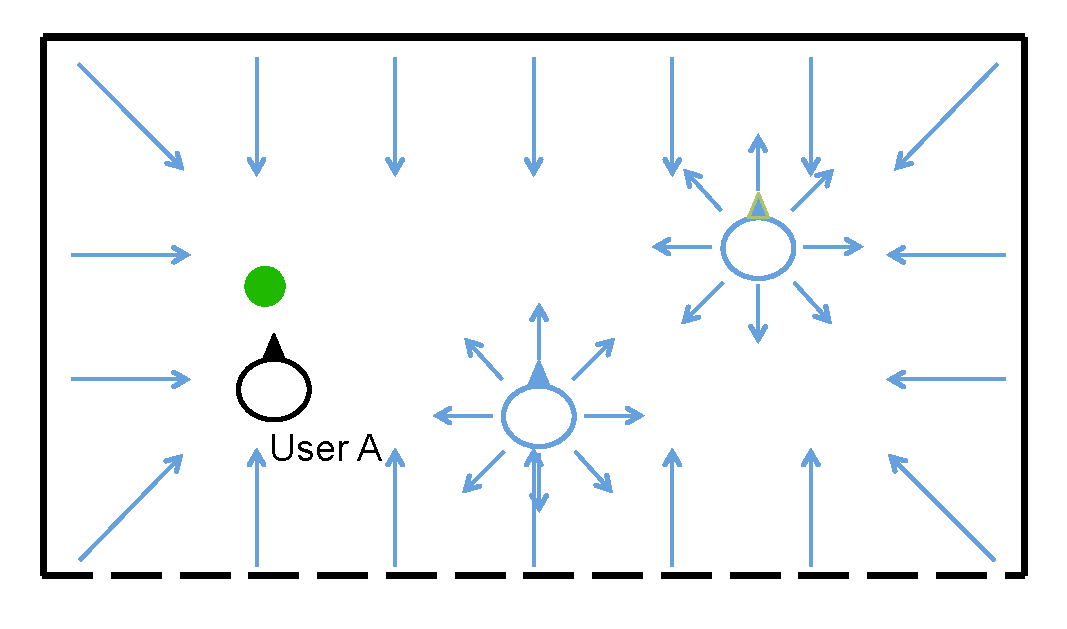
\includegraphics[width=.49\textwidth]{figures/ch5/pf_t_total}
  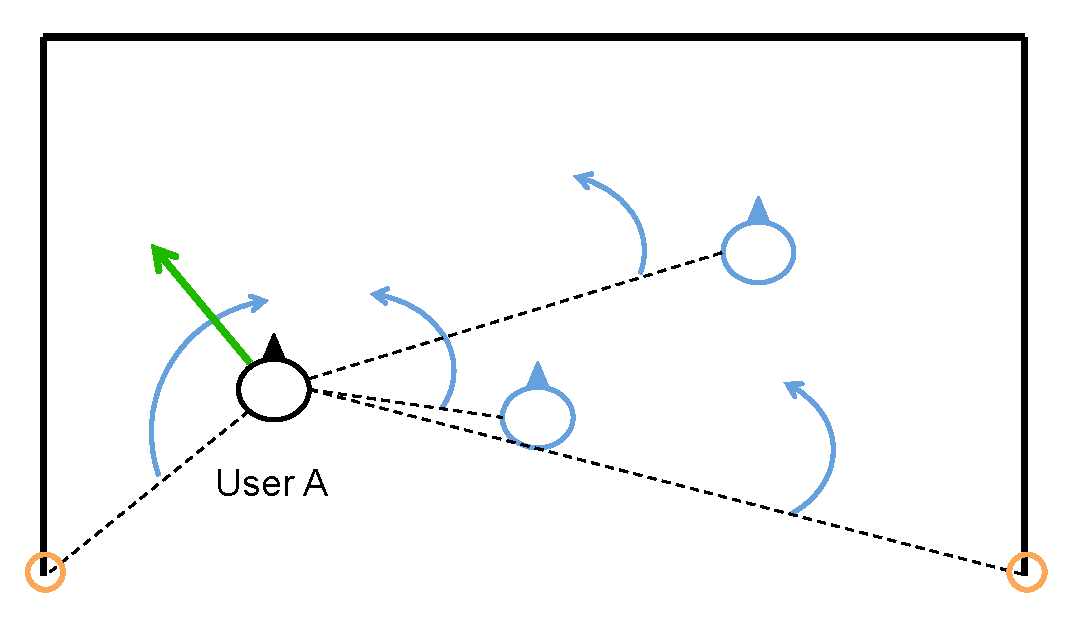
\includegraphics[width=.49\textwidth]{figures/ch5/pf_r_total}
  \caption{\label{fig:5_pf_total}The global translational and rotational potential field for user A in a three-wall CAVE.}
\end{figure}


To find the optimal configuration for a user in real time, we used an iterative method as presented in Algorithm~\ref{algo:optimal_point}. The idea is to create a virtual position $p$ (orientation $q$) starting from user's current position $p_{u}$ (orientation $q_{u}$) and pushed (rotated) by the sum of all force vectors step by step till we reach a certain precision $\epsilon_{T}$ ($\epsilon_{R}$) and and round number $n_{T}$ ($n_{R}$). This allows us to find the optimal position and orientation for each user during a rendering frame.

\begin{algorithm}[htb]
\caption{Iterative function for optimal configuration computing.}
\label{algo:optimal_point}
\begin{algorithmic}
\REQUIRE $\epsilon_{T} \geq 0 \: \AND \: n_{T}>0 \: \AND \: \epsilon_{R} \geq 0 \: \AND \: n_{R}>0$
\STATE $p \leftarrow p_{u}$
\STATE $p_{opt} \leftarrow p+\sum \overrightarrow{ft}_{i}$
\STATE $round \leftarrow 0$
\WHILE{$|p_{opt}-p|>\epsilon_{T} \: \AND \: round<n_{T} \:$}
\STATE{$p \leftarrow p_{opt}$}
\STATE{$p_{opt} \leftarrow p+\sum \overrightarrow{ft}_{i}$}
\STATE{$round \leftarrow round+1$}
\ENDWHILE

\STATE $q \leftarrow q_{u}$
\STATE $q_{opt} \leftarrow q \cdot \sum fr_{i}$
\STATE $round \leftarrow 0$
\WHILE{$(q^{-1}_{opt} \cdot q).angle>\epsilon_{R} \: \AND \: round<n_{R} \:$}
\STATE{$q \leftarrow q_{opt}$}
\STATE{$q_{opt} \leftarrow q \cdot \sum fr_{i}$}
\STATE{$round \leftarrow round+1$}
\ENDWHILE
\RETURN $p_{opt}, q_{opt}$
\end{algorithmic}
\end{algorithm}


As the potential fields constantly push users towards their optimal configurations, we can use the difference between user's current configuration and corresponding optimal configuration to modify user's navigation control. Here we got two options:

\paragraph{Option 1: Scaling}
We can use the difference to scale user's input. For translation, the difference can be represented by a vector $\overrightarrow{d}$ pointing from the optimal position to user's current position. By splitting user's velocity $\overrightarrow{v_{u}}$ (and acceleration $\overrightarrow{a_{u}}$) to different axis, these components can then be scaled by the corresponding components of $\overrightarrow{d}$:   

\begin{equation}
\overrightarrow{v'_{ui}}=\overrightarrow{v_{ui}} \cdot (1+\frac{\overrightarrow{v_{ui}} \cdot \overrightarrow{d_{i}}}{|\overrightarrow{v_{ui}} \cdot \overrightarrow{d_{i}}|} \cdot K_{ot} \cdot |\overrightarrow{d_{i}}|), \;i\in\{x ,y\}
\end{equation}

where $K_{ot}$ is a coefficient to increase or reduce the influence of potential field. When $\overrightarrow{v_{ui}}$ is in the same direction with $\overrightarrow{d_{i}}$, the final input $\overrightarrow{v'_{ui}}$ will be amplified compared to $\overrightarrow{v_{ui}}$, otherwise it will be reduced (Figure~\ref{fig:5_option1:t}).

Similarly, for rotational control, we use $\theta$ to represent the angle between user's optimal orientation $q_{opt}$ and current orientation $q_{u}$. The angular velocity will be amplified if the user turns away from $q_{opt}$, otherwise it is reduced to encourage user's turn faster towards $q_{opt}$ (Figure~\ref{fig:5_option1:r}).

\begin{equation}
\omega'_{u}=\omega_{u} \cdot (1+sign \cdot K_{or} \cdot \theta),\;sign \in \{-1, 1\} 
\end{equation}

where $sign$ is computed depending on the relationship between user's angular velocity and the rotation direction starting from $q_{opt}$ to $q_{u}$. $K_{or}$ also serves as a scale factor like $K_{ot}$. Both $K_{ot}$ and $K_{or}$ are set small enough so the potential field will not inverse the direction of user's input.

\begin{figure}[htb]
  \begin{subfigure}{.5\textwidth}
    \centering
    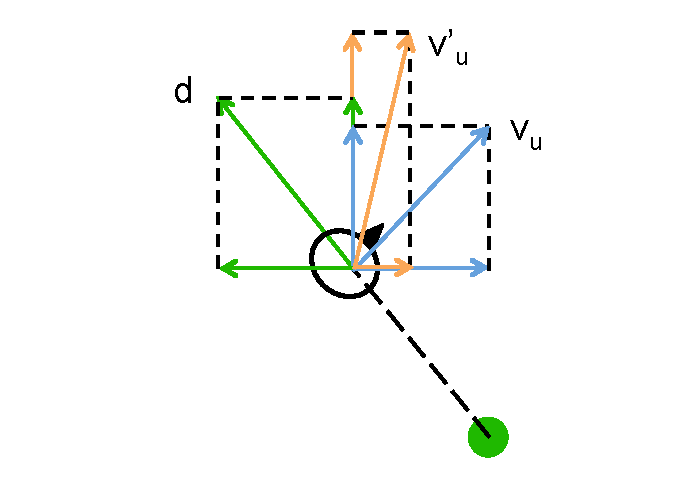
\includegraphics[height=5cm]{figures/ch5/option1_t}
    \caption{Velocity vectors are scaled by $\overrightarrow{d}$.}
    \label{fig:5_option1:t}
  \end{subfigure}
  \begin{subfigure}{.5\textwidth}
    \centering
    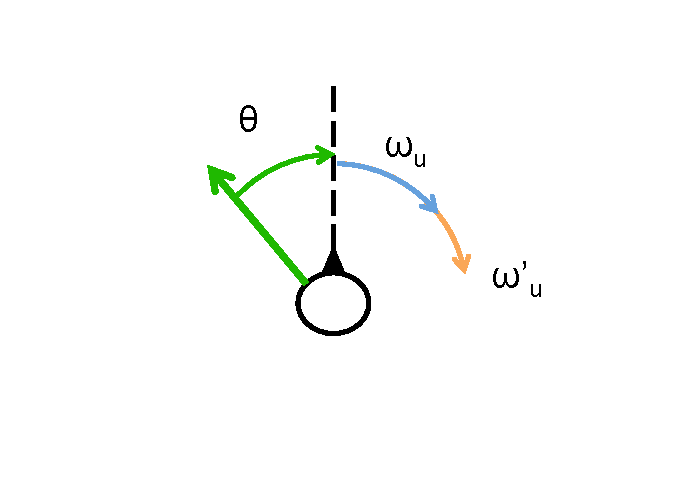
\includegraphics[height=5cm]{figures/ch5/option1_r}
    \caption{Angular velocity is scaled by $\theta$.}
    \label{fig:5_option1:r}
  \end{subfigure}
  \caption{\label{fig:5_option1}Scaling of user's input by the difference between user's current configuration and the optimal configuration.}
\end{figure}

\paragraph{Option 2: Acceleration Insertion}
Instead of scaling user's input, we can also insert additional accelerations to ``pull" users towards the optimal configuration. We can consider that the user and optimal configuration are connected by a mass spring damper system (a PD system in automatics which is useful to represent interconnection between two mobile entities). For translation, the total acceleration is the sum of acceleration coming from the transfer function $\overrightarrow{a_{u}}$ and $\overrightarrow{a_{o}}$ generated by the optimal position (Figure~\ref{fig:5_option2:t}). $\overrightarrow{a_{o}}$ is expressed as follows:

\begin{equation}
\overrightarrow{a_{o}}=K_{ot} \cdot (p_{u}-p_{o})+ B_{ot} \cdot (\overrightarrow{v_{u}}-\overrightarrow{v_{o}})
\end{equation}

where $K_{ot}$ and $B_{ot}$ are respectively spring and damper coefficients, $p_{o}$ and $\overrightarrow{v_{o}}$ are the position and velocity of the optimal configuration.

For rotation, the total angular acceleration $\dot{\omega}_{total}$ is the sum of $\dot{\omega}_{u}$ and $\dot{\omega}_{o}$ (Figure~\ref{fig:5_option2:r}). $\dot{\omega}_{o}$ is expressed as follows:

\begin{equation}
\dot{\omega}_{o}=K_{or} \cdot (q_{u}-q_{o})+ B_{or} \cdot (\omega_{u}-\omega_{o})
\end{equation}

where $K_{or}$ and $B_{or}$ are respectively spring and damper coefficients, $q_{o}$ and $\omega_{o}$ are the optimal orientation and its rotational velocity.

\begin{figure}[htb]
  \begin{subfigure}{.5\textwidth}
    \centering
    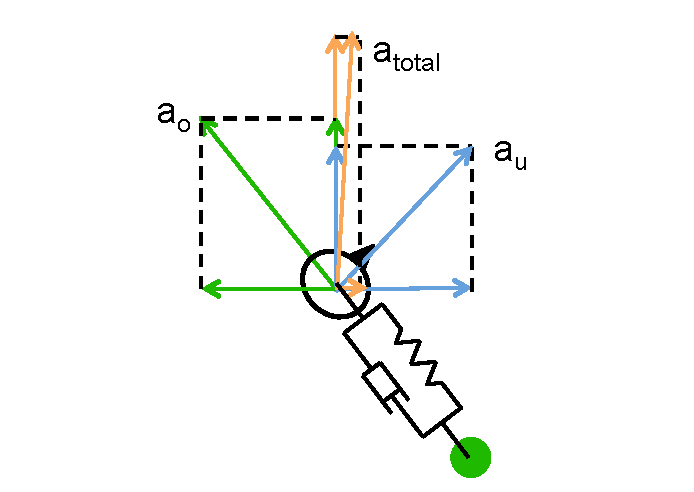
\includegraphics[height=5cm]{figures/ch5/option2_t}
    \caption{Additional linear acceleration $\overrightarrow{a_{o}}$.}
    \label{fig:5_option2:t}
  \end{subfigure}
  \begin{subfigure}{.5\textwidth}
    \centering
    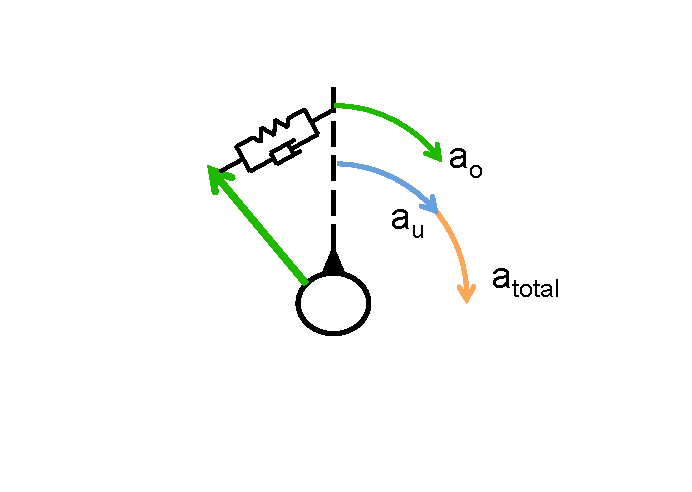
\includegraphics[height=5cm]{figures/ch5/option2_r}
    \caption{Additional angular acceleration $\dot{\omega}_{o}$.}
    \label{fig:5_option2:r}
  \end{subfigure}
  \caption{\label{fig:5_option2}Inserting additional accelerations by the difference between user's current configuration and the optimal configuration.}
\end{figure}

\paragraph{Comparison}
These two options give users similar navigation experiences in terms of perceived acceleration as they are both based on the difference between user's current configuration and the optimal configuration decided by the potential field distribution. The major difference is that option 2 continues to accelerate the navigation as long as the user is not at the optimal configuration, so normally users are never far away from their optimal configurations, while with option 1 the vehicle is accelerated only when the user intends to, but we can not assure that the user always stays at the optimal configuration.

\subsubsection{Command Configuration}
Since users are mobile in the physical workspace, the potential field for each user is changing all the time depending on the positions of other users, the movements of one user change instantaneously the optimal configuration of another, which will induce instability to the navigation control, especially for option 2.

To reduce this instability, a possible solution is to define a command configuration $c_{command}$ as an intermediate layer between $c_{u}$ and $c_{opt}$. The $c_{command}$ indicates where the user should be in the real world and tries to join $c_{opt}$ with a certain delay. For example, we can create a mass spring damper link between $c_{command}$ and $c_{opt}$ to reduce the influence of $c_{opt}$ on the virtual vehicle.

Moreover, the optimal configuration defined by the potential field may not always be the preferred destination, we may have some other real world constrains to take into account. For example, a user may need to leave more workspace for another user based on their individual task requirements. So the command configuration is useful as a higher abstraction level for us to integrate other real world constrains besides obstacles' potential fields. 


\subsection{Virtual World Constrains}
Unlike in 

In the dynamic navigation model, 


\subsubsection{Interaction with Environment}
interaction with virtual world
 - simulate physical behavior         we can apply an acceleration in the opposite direction of the vehicle's current velocity to
                                     simulate the viscosity or friction of the virtual world

 - integrate with physics engine      cross wall: collision

\subsubsection{Interaction between Users}
interact with other user             

three levels of user interaction
Imagine two users moving together a virtual table to another place, in this case their vehicles are virtually connected by the table so they have mutual influences on each other's navigation control

% -------------------------------------------------------------------------------------------------


\section{Implementation}
\subsection{Kinematic State}
Kinematics is a field of study which describes the motion of points and more complex objects without consideration of the causes of motion \citep{Beggs1983Kinematics}. It is the basic component of a physics engine for virtual simulation.

Instead of navigating by setting a user's position and orientation in the virtual world, we can also make use of other kinematic information such as velocity and acceleration to control user's virtual motion, especially in cases where we look for navigation sensations that are close to those we have in the physical world. 

\subsubsection{Representation}
We created a variable called \textit{kinematic state} (KS) to store all motion-related data of a given object. In 3D space, an object's KS usually contains two parts of information respectively for translation and rotation, except those of points (considered as particles) which have only positional information. Different components of an object's KS are listed in Table~\ref{tab:5_ks_components}.

\begin{table}[hbt]
\renewcommand{\arraystretch}{1.3}
\caption{Components of kinematic state}
\label{tab:5_ks_components}
\centering
\begin{tabular}{l l l}
  \hline
  Components & Translation Part & Rotation Part \\
  \hline
  Static configuration $c(p, q)$ & Position $p(x, y, z)$ & Orientation $q(w, x, y, z)$ \\
  Velocity $v(\overrightarrow{v}, q_{v})$ & Linear velocity $\overrightarrow{v}(v_{x}, v_{y}, v_{z})$ & Angular velocity $q_{v}$ \\
  Acceleration $a(\overrightarrow{a}, q_{a})$ & Linear acceleration $\overrightarrow{a}(a_{x}, a_{y}, a_{z})$ & Angular acceleration $q_{a}$ \\
  \hline
\end{tabular}
\end{table}


\subsubsection{State Update}
An object's KS changes constantly while moving in 3D space. The current KS can be updated by providing a new acceleration, or by directly designing a new static configuration. For example, we can accelerate a virtual object by injecting an acceleration on that object, this results in a corresponding velocity and configuration change. A real world entity such as a user's physical body also has a KS,

 The user also has a KS that is updated by tracking information in a different way than the vehicle.

\paragraph{Update by Acceleration}
The verlet integration is used to update the KS with a new acceleration.

For translation:

\[
\overrightarrow{p_{1}}=\overrightarrow{p_{0}}+\overrightarrow{v_{0}}\Delta t+\frac{1}{2}\overrightarrow{a_{0}}\Delta t^{2}
\]

\[
\overrightarrow{v_{1}}=\overrightarrow{v_{0}}+\frac{\overrightarrow{a_{0}}+\overrightarrow{a_{1}}}{2}\Delta t
\]

And for rotation, we choose to represent the orientation in quaternion for its convenience and simplicity, while angular velocity and acceleration are expressed separately according to euler angles:

\[
\omega_{1}=\omega_{0}+\frac{\dot{\omega_{0}}+\dot{\omega_{1}}}{2}\Delta t
\]

\[
q_{1}=q_{a}q_{v}q_{0}
\]

\[
q_{v}=\left(\cos(\frac{\Vert\omega_{0}\Vert\Delta t}{2}),\:\sin(\frac{\Vert\omega_{0}\Vert\Delta t}{2})\frac{\omega_{0}(x)}{\Vert\omega_{0}\Vert\Delta t},\:\sin(\frac{\Vert\omega_{0}\Vert\Delta t}{2})\frac{\omega_{0}(y)}{\Vert\omega_{0}\Vert\Delta t},\:\sin(\frac{\Vert\omega_{0}\Vert\Delta t}{2})\frac{\omega_{0}(z)}{\Vert\omega_{0}\Vert\Delta t}\right)
\]

\[
q_{a}=\left(\cos(\frac{\Vert\dot{\omega_{0}}\Vert\Delta t}{2}),\:\sin(\frac{\Vert\dot{\omega_{0}}\Vert\Delta t}{2})\frac{\dot{\omega_{0}}(x)}{\Vert\dot{\omega_{0}}\Vert\Delta t},\:\sin(\frac{\Vert\dot{\omega_{0}}\Vert\Delta t}{2})\frac{\dot{\omega_{0}}(y)}{\Vert\dot{\omega_{0}}\Vert\Delta t},\:\sin(\frac{\Vert\dot{\omega_{0}}\Vert\Delta t}{2})\frac{\dot{\omega_{0}}(z)}{\Vert\dot{\omega_{0}}\Vert\Delta t}\right)
\]


\paragraph{Update by Configuration}
(in form of a 4x4 matrix)



\subsection{Structure}

python

class schema

sequential graph

a solver

An \textbf{Inverse Model} computes an acceleration based on the difference between the command point and user's current configuration which helps to lead the user to that point.



% -------------------------------------------------------------------------------------------------

\section{Discussion}
Parameter Setting user perception

One user should not be disturbed by other users when in a stable state

% -------------------------------------------------------------------------------------------------

\section{Conclusion}
We need a model of human for reaction of acceleration.